\section{Visualization of a day of a programmer}\label{sec:vis}

I present two visualizations (as plots): using \texttt{additions}/\texttt{deletions} \ref{fig:add_and_del_vis} and \texttt{actions} \ref{fig:actions_vis}. Both of them show the values of their respected attributes per unit of time. This way it is easier to consider programmer's features such as his performance. The first visualization makes it possible to analyze the programmer's working day in a more sophisticated way. The numbers of added or deleted characters may indicate the actual tasks done by the developer (i.e. writing, editing or removing parts of the codebase) in the relevant time periods. The second visualization focuses on providing an approximate image of programmer's performance, since \texttt{actions} per second can be interpreted as a simple metric of this feature.

\begin{figure}[htbp]
  \centering
  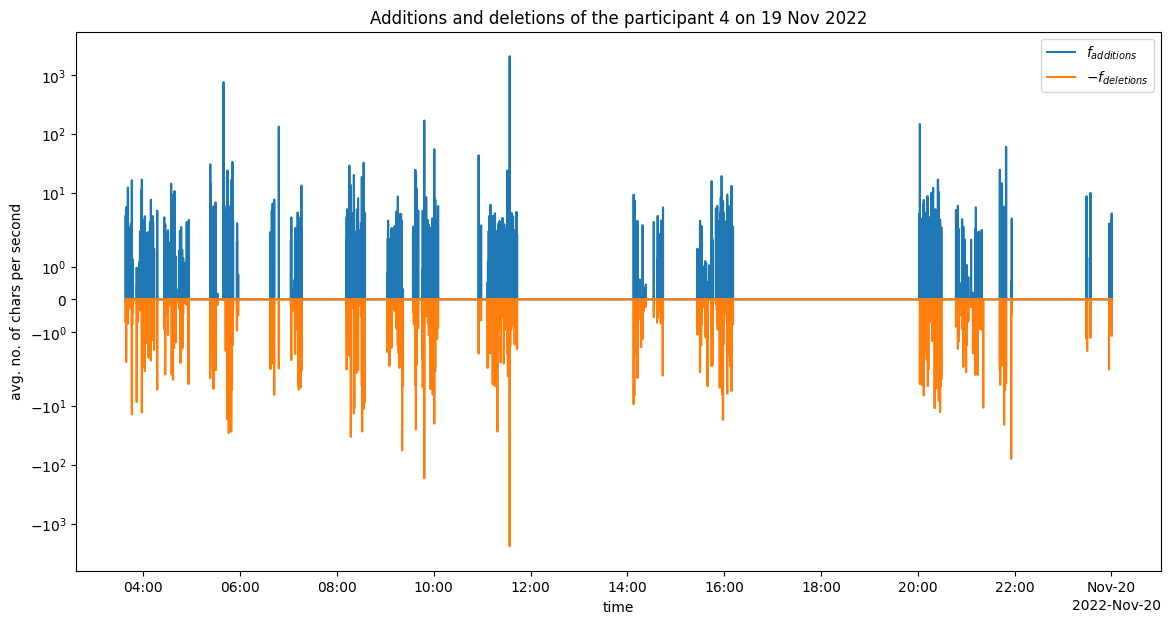
\includegraphics[scale=0.5]{chapters/results/graphics/add-and-del-vis.png}
  \caption{Visualization of a programmer's day with \texttt{additions} and \texttt{deletions}}
  \label{fig:add_and_del_vis}
\end{figure}

\begin{figure}[htbp]
  \centering
  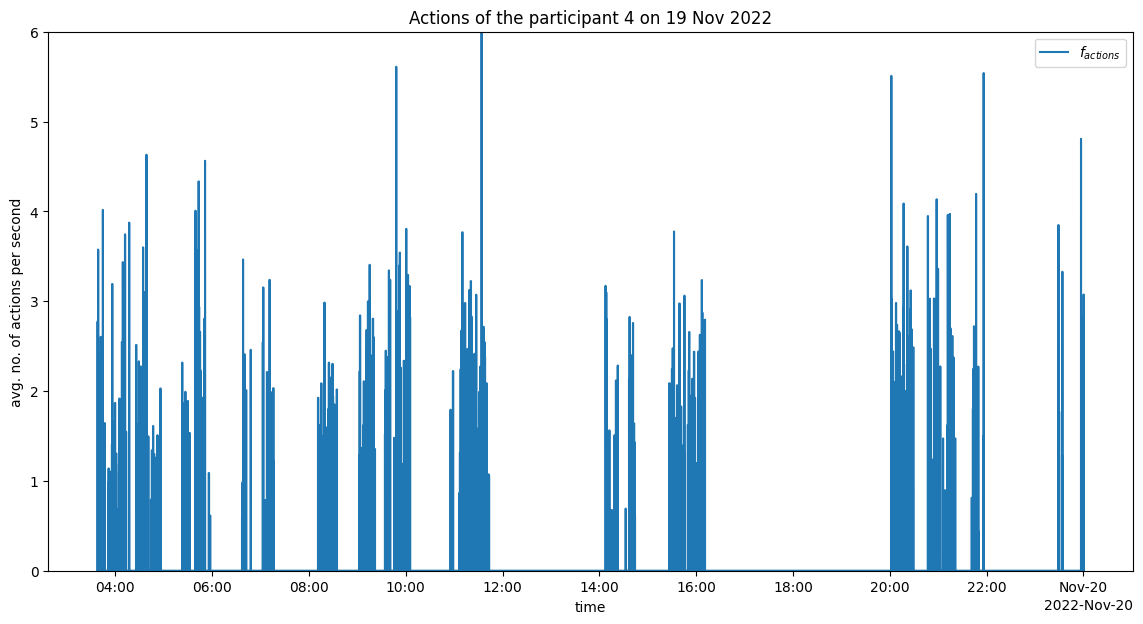
\includegraphics[scale=0.5]{chapters/results/graphics/actions-vis.png}
  \caption{Visualization of a programmer's day with \texttt{actions}}
  \label{fig:actions_vis}
\end{figure}
